{\textbf{1. 三种离散分配方式的比较}}

在内存管理方式中,离散分配管理方式比连续分配管理方式重要得多,而且也是历年研究生考试的考查重点,因此将三种离散分配方式单独拿出来进行比较,见下表。

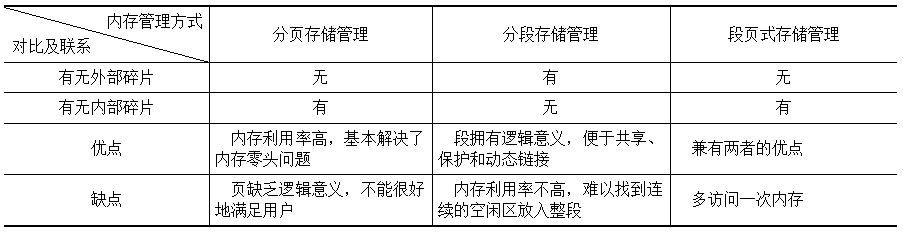
\includegraphics[width=3.33333in,height=0.86458in]{png-jpeg-pics/74DB87F60323C7B2370478B20D9E3968.png}

\textbf{{2. 几种内存管理方式之间的比较}}

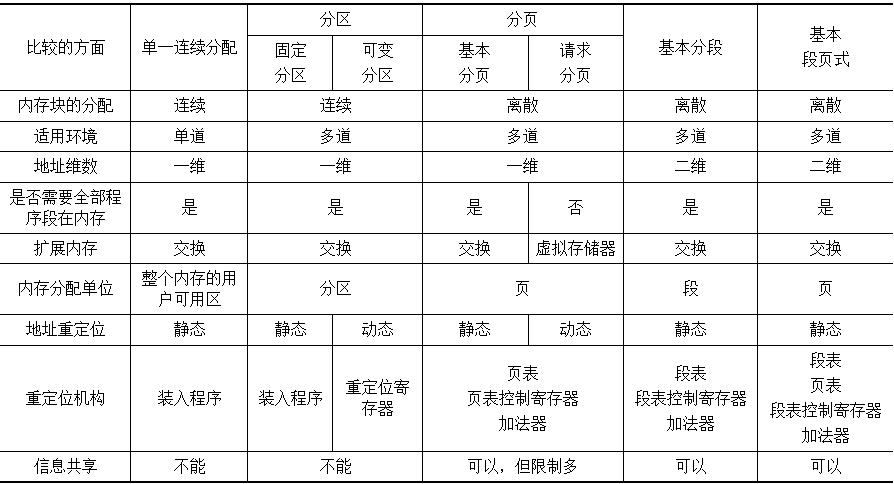
\includegraphics[width=3.33333in,height=1.80208in]{png-jpeg-pics/87FB39189D2C90C64F4D1EBEAF5127FE.png}
